\chapter{Fundamentos de Robótica e Planejamento de Trajetória}
\label{chap:fundam}

\section{Planejamento de trajet\'oria}

O objetivo principal da zona de planejamento de trajetória é a construção de algoritmos para automatizar o movimento de robôs, 
peças e outros ambientes que utilizam objetos geométricos arbitrários. A tarefa básica é mover um robô em seu ambiente de trabalho 
a partir de uma posição e orientação para outra posição e orientação desejada, sem o robô bater em obstáculos. O planejamento de 
movimento tem aplicações tanto dentro como fora da área de robótica.

O problema de navegação mais básico é mover um robô modelado como um ponto no espaço através de um ambiente bidimensional com vários
itens proibidos (ou obstáculo ), as regiões que o robô não pode entrar. O modelo é cinemático, o que significa que a única limitação
é que o robô tem de se mover ao longo de uma trajetória contínua.

O robô é modelado como um ponto no espaço de configuração, em vez de o espaço de trabalho. Uma configuração é uma especificação
do local (localização e orientação) do robô em relação ao meio ambiente e o espaço de configuração é o conjunto de todas as configurações
possíveis \cite{achoset}.

Realizar o planejamento apresenta um maior nível de complexidade quando o robô tem muitos graus de liberdade e orientação. Um robô 
guia pode passar por um espaço com uma certa posição e orientação, e atinge um obstáculo se fosse em uma orientação diferente. Isso 
aumenta a complexidade dos algoritmos para planejamento de trajetória.

O exemplo clássico de planejamento de trajetória é o problema do mecanismo de enfileiramento \cite{bsharir}: 
mover um piano através de uma casa de piano para não colidir com outros objetos na casa (ou a própria casa). Apenas considerou a 
geometria dos objetos e não as forças que atuam sobre o piano, como a gravidade .

Estendendo a analogia, o piano é suposto ter motores infinitamente fortes e infinitamente pequeno. Portanto, o problema do motor 
de piano só lida a circulação de uma forma geométrica ao longo de um caminho que é contínuo no espaço através de uma atmosfera.

Finalmente, talvez o mais difícil de restrição está relacionada com a estética do movimento. Pode ser desejável, para os movimentos 
do robô, para imitar o movimento humano. Por estas razões, os métodos baseados em amostra, não parecem ser a solução para o planejamento
de movimento humanóide.

Existem diversos algoritmos que tratam da navegação de agentes humanóides, sendo que um dos primeiros é descrito no livro de
Inteligência Artificial de Russell e Norvig, o algorítmo A* \cite{brussel}. Ele busca o caminho em um grafo de
um vértice inicial até um vértice final, é a combinação de aproximações heurísticas como do algoritmo Best-first Search e da
formalidade do Algoritmo de Dijkstra (DIJKSTRA, 1959). 

A partir do algoritmo A*, surgiram derivações como o R*\cite{plikhachev}, que depende muito menos da qualidade da função heurística, 
evitando mínimos locais e resolvendo o problema de planejamento de toda uma série de pesquisas de curto alcance.

\section{Algorítmo R*}

Pesquisas heurísticas ótimas, como uma pesquisa A* são amplamente usadas para planejamento, mas raramente podem escalar para grandes problemas complexos. 
As versões sub-ótimas de buscas heurísticas, tais como pesquisa A*, muitas vezes podem ser escaladas para problemas de planejamento maiores, trocando 
a qualidade da solução para a eficiência. Elas fazem isso contando mais com a capacidade da função heurística para orientá-los bem para o gol. Para
problemas complexos de planejamento, no entanto, a função heurística muitas vezes pode orientar a busca em um grande mínimo local e fazer a busca 
examinar a maioria dos estados no mínimo local antes de prosseguir.

A busca heurística, denominada Busca R*\cite{plikhachev}, depende muito menos da qualidade da função heurística. A busca evita mínimos locais, resolvendo
o problema de planejamento de toda uma série de pesquisas de curto alcance e fácil de resolver, cada um guiado pela função heurística para um objetivo
escolhido aleatoriamente. Além disso, muitas escalas R* são melhores em termos de memória, pois podem descartar uma pesquisa no espaço-estado após 
cada uma de suas pesquisas. O algoritmo possui garantias probabilísticas em sub-otimização da solução devolvido por R* e pode ser dimensionado para
grandes problemas complexos.

Em vez de executar uma única pesquisa focada no sentido de um estado meta, R* tenta executar uma série de buscas ponderada A* de curto alcance no sentido 
de escolher estados meta aleatoriamente e reconstruir uma solução dos caminhos produzido por essas pesquisas. A principal idéia por R* baseia-se que ao 
invés de executar cada uma de suas pesquisas de curto alcance até que encontre soluções, R* adia os que não encontram soluções facilmente e tenta construir
a solução global usando apenas os resultados das pesquisas que encontrar soluções facilmente. 

%Rever a traducao dessa parte, está estranho
Programações e reprogramações de pesquisas de curto alcance são formas de dar garantias probabilísticas na sub-otimização da solução global que encontra. 
O algoritmo também possui sub-otimização ao segurar com probabilidade igual a 1 se R* não realiza down-select randomizado, do que agendar pesquisas de curto 
alcance. O algoritmo pode encontrar soluções para esses problemas com muito mais frequência do que pesquisa ponderada A*, e pode minimizar o custo de
encontrar soluções muito melhores do que os algoritmos de planejamento de movimento ao acaso, desenvolvidos especificamente para domínios contínuos.

\section{Geração de marcha}
Devido à complexidade do problema de planejamento de trajetórias, os investigadores e engenheiros frequentemente concentram-se 
em gerar movimentos curtos, tais como um único passo, ou repetindo andamentos em um ambiente livre de obstáculos. Este problema 
de geração de marcha é a segunda dificuldade núcleo de planejamento de movimento para caminhar robôs.

Sistemas mecânicos do andar de um robô não são facilmente controladas. Um robô andando tem uma dinâmica de sistemas não-lineares. 
Este sistema de equações terá apenas uma pequena gama de trajetórias que mantêm robô caindo, uma exigência da estabilidade, e as 
entradas de controle para o sistema será limitado como os motores só podem exercer um torque de até algum valor máximo. Este modelo 
matemático é geralmente difícil de analisar e não pode mesmo ter, uma solução explícita de forma fechada. Mesmo ignorando a geometria 
do ambiente, métodos de geração de marcha devem levar em consideração as colisões entre os elos do robô (auto-colisões). Além disso, 
as dificuldades de modelagem adicionais entram em jogo. O contato entre o pé de apoio do robô  e o solo não é um conjunto perfeito. O 
pé de apoio pode escorregar em momentos em que ela não deve se mover, e o atrito pode fazer mover-se difícil um pé de apoio. Além 
disso, o modelo deve considerar a força de impacto aplicada ao pé nos primeiros contatos do robô no solo e as forças de fricção na articulação.

Este problema da geração de marcha não é simples. Um número de abordagens são comumente feitas. Uma abordagem é desenvolver uma marcha
e projetar um controlador para controlar um padrão de movimentos articulares. Andamentos são gerados manualmente em alguns casos, pela
intuição de um designer humano ou por meio de captura de movimento para imitar diretamente o movimento humano \cite{bchoi}. 

Embora estes métodos dependem muito de uma trajetória predefinida, uma segunda abordagem baseia-se fortemente no feedback para 
estabilizar o robô. Políticas de controle com base no ponto do momento zero  do robô \cite{pkajita} \cite{pnagasaka} são exemplos comuns 
desta metodologia. Ao olhar e controlar os indicadores de comportamento do sistema, tais como o centro de massa, centro de pressão, 
ou ponto de momento zero, os controles que são projetados produzem (tipicamente) gerações estaticamente estáveis.

Apesar de não serem obrigados a seguir uma trajetória específica, estes métodos de feedback, especialmente de ponto de momento zero,
são em grande parte de energia ineficiente. Os custos do transporte (COT) é uma medida da eficiência de conversão de um sistema 
mecânico de energia para locomoção. Essencialmente, é a quantidade de energia consumida dividido pelo peso e pela distância percorrida
\cite{bkuo}. Por exemplo, o Asimo , da Honda , que utiliza o controle ponto de momento zero, tem um COT de 3,2 , que é 
cerca de dez vezes o COT de um ser humano.

Uma fusão de ambos geração marcha e planejamento de trajetória é útil para o planejamento de movimento bípede. Ambos planejamento de 
trajetória e métodos de geração de marcha têm desvantagens. No entanto, quando combinados de uma forma coordenada, eles podem amplificar 
sucessos um do outro enquanto parcialmente atenuar as deficiências do outro.

\section{Abordagem H\'ibrida}
Levando em considera\c{c}\~ao que o planejamento de trajet\'oria e problemas de controle s\~ao conhecidos por serem dif\'iceis, 
tanto analiticamente e computacionalmente, algumas abordagens para a navega\c{c}\~ao de rob\^os human\'oides s\~ao baseadas em 
uma simplifica\c{c}\~ao do modelo de planejamento de movimento human\'oide.

Planejamento de trajetória para um robô humanóide em terreno plano pode ser considerado como uma busca por uma seqüência de movimentos
primitivos vi\'aveis ao inv\'es de uma busca de um espa\c {c}o de configura\c{c}\~ao dimensional elevado para uma trajetória \cite{bkuffner}. 
O algoritmo de busca pode, em muitos casos, encontrar rapidamente uma seqüência de movimentos para levar o robô para o seu destino. No entanto,
a pesquisa vai exigir exponencialmente mais cheques como o número de primitivas de movimento naquele caminho. Em ambientes com obstáculos, 
escadas, rampas e buracos , os movimentos de humanóides são constrangidos por mais do que apenas a colocação do robô no plano. Um grande 
conjunto de primitivas de movimento é necessário para atravessar esses ambientes. Um algoritmo de programação dinâmica, uma pesquisa * ou
para frente pode levar um tempo considerável para calcular uma seqüência de primitivas de movimento ou o problema pode tornar-se 
computacionalmente intratável. Algumas abordagens de planeamento hierárquicos têm sido aplicados para controlar o crescimento de complexidade 
e encontrar uma solução para este problema aproximado \cite{pchesnutt}.

\section{Planejamento de Passo}
O planejamento de passo eficiente para navegação humanóide através de ambientes desordenados ainda é um problema desafiador. Muitos obstáculos
criam mínimos locais no espaço de busca, forçando planejadores heurísticos, tais como o A* para expandir grandes áreas.

Abordagens populares de cálculo de passo eficiente para trajetórias dado um conjunto finito de ações com passo eficiente que são executáveis
pelo robô para fazer a busca de caminhos livres de colisão tratável. Um controlador de pé, em seguida, calcula a trajetória do angulo das juntas 
para caminhar nos passos planejados. A pesquisa no espaço de estados de passos fica realizada ou usando um método baseado no A* incluindo variantes dinâmicas 
\cite{phornung} \cite{pgarimort} ou métodos randomizados\cite{bperrin}. Enquanto o A* vai encontrar o caminho ideal para parametrizção de um 
determinado passo e discretização do estado, o seu desempenho depende fortemente da qualidade da função heurística que orienta a pesquisa, mais não 
tem quaisquer garantias sobre a qualidade da solução do caminho final. Além disso, muitas vezes eles dependem do alisamento do caminho 
final em um fase de pós-processamento.

Este método leva inerentemente a capacidade de robôs humanóides para passar por cima de obstáculos. Um conjunto discreto de
transições de passo, ilustrado na figura \ref{fig:footstep}, é utilizado em uma heurística de busca tais como A*\cite{bperrin}. Por este meio, estados 
constituem a posição e orientação $( x, y, \theta )$ do pé de apoio atual. O próximo estado pode ser alcançado através da aplicação da ação de 
um dos passos possíveis e mudando o pé de apoio.

\begin{figure}[h]

\centering

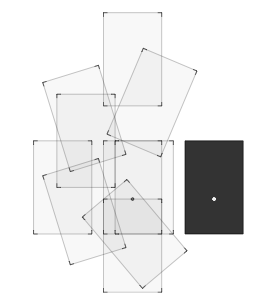
\includegraphics[scale=0.48]{figuras/footstep.png}

\caption{Parametrização do passo para um humanóide com dez etapas diferentes, mostrado como deslocamentos do pé esquerdo em 
relação ao pé de suporte direito.} Fonte: \cite{phornung} \label{fig:footstep}

\end{figure}
\FloatBarrier

A partir do estado inicial, o planejador sucessivamente adiciona transições de passos, a fim de encontrar o caminho mais eficiente para o gol. 
Os custos de transição são dados pelo custo de execução do passo correspondente, isto é, são baseadas com a distância que o passo cobre e um 
custo constante, a fim de favorecer caminhos com menos etapas. Cada novo estado é checado para colisões e é descartado se for colidir com 
obstáculos. Caso contrário, o planejador se expande ainda mais, investigando as próximas transições. A busca fica guiada por uma heurística
que ajuda a concentrar-se nos estados promissores para o objetivo.

Uma das heurísticas comuns para o passo de planejamento é usar o distância em linha reta para o gol, ou os custos estimados ao longo de um caminho 2D 
planejado com A*. O último é potencialmente inadmissível uma vez que não reflete a capacidade do humanóide passando por cima de obstáculos.
Na prática, contudo, o caminho resultante é geralmente não menos eficiente e significativamente mais rápido computar como as heurísticas
que orienta a pesquisa mais focada para o objetivo \cite{pgarimort}. Em contraste com o planejamento de caminho 2D padrão,
planejamento de passos leva também a orientação dos estados em conta. O maior número de possíveis transições de estado e as verificações de 
colisão mais complexas são as razões pelas quais planejamento de passo é computacionalmente mais exigente do que Planejamento de trajetória 2D.

\section{Futebol de Robôs}

\subsection{RoboCup}

A iniciativa RoboCup \cite{kitano95} \cite{Kitano97} é um projeto de investigação e educação internacional que tem como objetivo 
promover a investigação em Inteligência Artificial Distribuída e Robótica Inteligente \cite{robocup}. O projeto tem como base a 
utilização de um problema standard – o futebol robótico – onde o desenvolvimento de tecnologias para construir uma equipe de Robôs 
reais ou virtuais seja capaz de participar de um desafio de futebol seguindo regras de jogo pré-especificadas.
%OK

Como forma de promover a investigação na área, foi lançado um objetivo de longo prazo: 

“No ano de 2050, uma equipe de robôs autônomos humanóides, ser capaz de vencer a 
equipe campeã do mundo de futebol, em uma partida disputada de acordo com as regras da 
FIFA.” \cite{Kitano97} 
%OK

Este objetivo é atualmente partilhado como um dos grandes desafios da área da Inteligência Artificial e Robótica. 
Embora este desafio, à luz da ciência e tecnologia atuais, pareça altamente ambicioso, a colocação de objetivos científicos
bem definidos de longo prazo, tem sido, ao longo dos anos, uma forma de estimular o desenvolvimento científico \cite{robocup}. 
Além disso, os sub-objetivos que são colocados pela RoboCup através das ligas, convergem para alcançar o objetivo final.
%OK

\subsubsection{Ligas da RoboCup}
O futebol robótico inclui diversas ligas que se dividem em dois tipos: ligas robóticas (utilizando robôs pequenos, médios e 
humanóides) e a liga de simulação. O objetivo é fazer com que cada liga se concentre nos desafios propostos, dando ênfase em 
determinados tópicos necessários para fazer com que equipes de robôs possam disputar uma partida de futebol. Por exemplo, 
na liga de simulação, a ênfase é colocada na coordenação em SMA, enquanto na liga de robôs pequenos, a ênfase é colocada no 
controle rápido e preciso dos robôs e na liga de robôs médios, os tópicos mais importantes incluem a visão computacional, 
projeto electromecânico e auto-localização dos robôs.
%OK

A RoboCup Rescue \cite{kitano99} e o RoboCup Júnior \cite{sklar02} são também outras iniciativas associadas ao futebol robótico. 
O Rescue divide-se em robótica física e simulada e tem como objetivo estimular a aplicação da investigação realizada no futebol 
robótico, a domínios socialmente mais úteis, no caso, missões de salvamento e resgate em grandes catástrofes \cite{rescue01}. Já 
a RoboCup Júnior surgiu como uma forma de estimular os mais jovens a participar da RoboCup. A OBR (Olimpíada Brasileira de Robótica) 
é um dos eventos que promovem a inclusão de jovens em idade escolar a construir e colocar em funcionamento os seus robôs para 
realizar diversas tarefas.
%OK

\subsubsection{Xadrez Vs RoboCup}
Um desafio semelhante colocado aos investigadores em Inteligência Artificial no decurso das últimas 4 décadas, consistiu em 
construir um agente (programa) que fosse capaz de vencer o campeão mundial de Xadrez utilizando as regras oficiais da Federação
Internacional de Xadrez. Tal desafio mostrou a importância da existência de problemas standard em que diferentes metodologias e
avanços científicos podem ser comparados. 
%OK

Diversos algoritmos de pesquisa, arquiteturas de computadores e metodologias científicas foram desenvolvidos para este domínio. 
Em Maio de 1997, o computador Deep Blue da IBM \cite{deepblue} derrotou Gary Kasparov (o campeão humano de Xadrez) \ref{fig:deepblue}
, utilizando as regras oficiais do Xadrez. Com esta vitória, o desafio de 40 anos da Inteligência Artificial utilizando o Xadrez 
como domínio de aplicação ficou muito próximo de um final com sucesso. 
%OK

\begin{figure}[h]

\centering

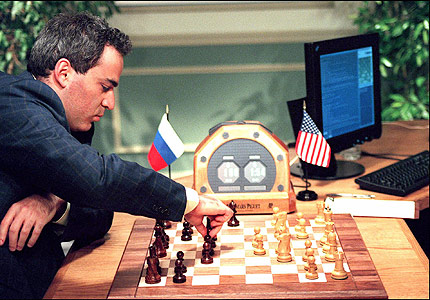
\includegraphics[scale=0.48]{figuras/deepblue.jpg}

\caption{Garry Kasparov x Deep Blue (Computador da IBM), jogando uma partida de Xadrez.} Fonte: \cite{flamencos} \label{fig:deepblue}

\end{figure}
\FloatBarrier


Uma das características que tornou o Xadrez computadorizado um problema standard foi a facilidade que este domínio ofereceu para
a comparação de abordagens distintas, e para a  avaliação do progresso científico global realizado no domínio. No entanto, com a
chegada ao final do desafio associado ao Xadrez, no mundo da IA, novos domínios e problemas standard mais complexos e estimulantes
tornaram-se necessários. Foi neste contexto que se desenvolveu o desafio do futebol robótico como um problema standard para a IAD 
e Robótica Inteligente. 
%OK

As principais diferenças entre o domínio do Xadrez e a RoboCup podem ser visualizadas na tabela \ref{tab:xadrobocup}.

\begin{table}[h]

\centering

\caption{Diferenças entre as características dos domínios do RoboCup e Xadrez.} Fonte: \cite{reisTese} 

  \begin{tabular}{|c|c|c|}

    \hline
    \hline
    Caracteristicas / Domínio & Xadrez & RoboCup \\
    \hline
    Ambiente & Estático & Diamico \\
    \hline
    Mudança de Estado & Por turnos & Tempo-Real \\
    \hline
    Acessibilidade ao Estado do Mundo & Completa & Incompleta \\
    \hline
    Resultado das Ações & Determinístico & Não Determinístico \\
    \hline
    Leitura dos Sensores & Discreta(Simbólica) & Contínua(não Simbólica) \\
    \hline
    Utilização dos Atuadores & Discreta(Simbólica) & Contínua(não Simbólica) \\
    \hline
    Controle & Centralizado & Distribuído \\
    \hline
    \hline
  \end{tabular}

  \label{tab:xadrobocup}
\end{table}

A RoboCup foi desta forma projetada de forma a colocar num mundo limitado, um conjunto elevado de complexidades do mundo real, 
mantendo no entanto o custo, complexidade global e dimensão do problema, acessível aos grupos de investigação em Robótica e 
Inteligência Artificial. Tais problemas de investigação colocados pela RoboCup de uma forma integrada, cobrem uma vasta área dos 
domínios da IA e Robótica, incluindo: coordenação, cooperação e comunicação multi-agente, arquiteturas de agentes inteligentes, 
aprendizagem, planeamento em tempo-real, decisão estratégica e táctica, comportamento reativo, visão por computador, processamento
e análise de imagem, sistemas de locomoção e atuação, sistemas sensoriais, fusão sensorial em tempo-real, navegação, controle 
inteligente robótico e outros.

\subsection{Simulação 3D}


\subsection{Simspark}

SimSpark \cite{simspark} é um sistema de simulação de multi-agente para agentes em ambientes tridimensionais desenvolvido como
parte da iniciativa RoboCup. Seu objetivo é fornecer um alto grau de flexibilidade para a criação de novos tipos de simulações. 
Baseia-se em um quadro de aplicação flexível e esgota a idéia de componentes substituíveis ao longo de sua implementação. 

Em comparação com simuladores especializados, os usuários podem criar novas simulações utilizando uma linguagem de descrição de
cena. O SimSpark é uma ferramenta poderosa, pois abrange diferentes questões de investigação multi-agentes e é usado como o 
simulador oficial para a competição RoboCup Simulation League.

O rcssserver3d é o ambiente de competição oficial para o Soccer Simulation League em 3D na RoboCup. Ele implementa uma simulação
de futebol, onde duas equipes de até onze robôs humanóides podem jogar uns contra os outros. Esta configuração aparentemente 
simples representa um desafio para os implementadores de agentes em vários níveis. 

O modelo de robô utilizado na simulação nas competições é atualmente o NAO \ref{fig:naoColorido}. Contudo, a utilização de agentes
heterogeneos tem ganhado destaque na área científica, que agora querem criar modelos capazes de se adequarem a qualquer tipo de 
robô.

\begin{figure}[h]

\centering

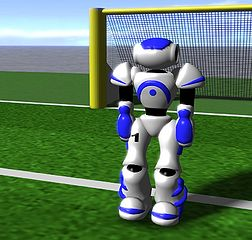
\includegraphics[scale=0.8]{figuras/naoColorido.jpg}

\caption{Simulação do Robô NAO da empresa Aldebaran Robotics feita pelo servidor oficial da liga 3D.} Fonte: \cite{SimulationLeague} \label{fig:naoColorido}

\end{figure}
\FloatBarrier
              
\subsection{Roboviz}

RoboViz \cite{roboviz} é um programa de software projetado para avaliar e desenvolver comportamentos do agente em um sistema 
multi-agente, a liga de futebol simulado RoboCup 3D. RoboViz é um monitor interativo que torna agente e informações sobre o 
estado do mundo em uma cena tridimensional. Além disso, o RoboViz fornece um design programável e funcionalidade de depuração
para os agentes que podem se comunicar através de uma rede. 

A ferramenta facilita a visualização em tempo real de agentes em execução simultânea no simulador SimSpark, e fornece uma análise
de nível superior e visualização de comportamentos do agente, que não está atualmente disponível nas ferramentas já existentes 
\ref{fig:roboviz}.

\begin{figure}[h]

\centering

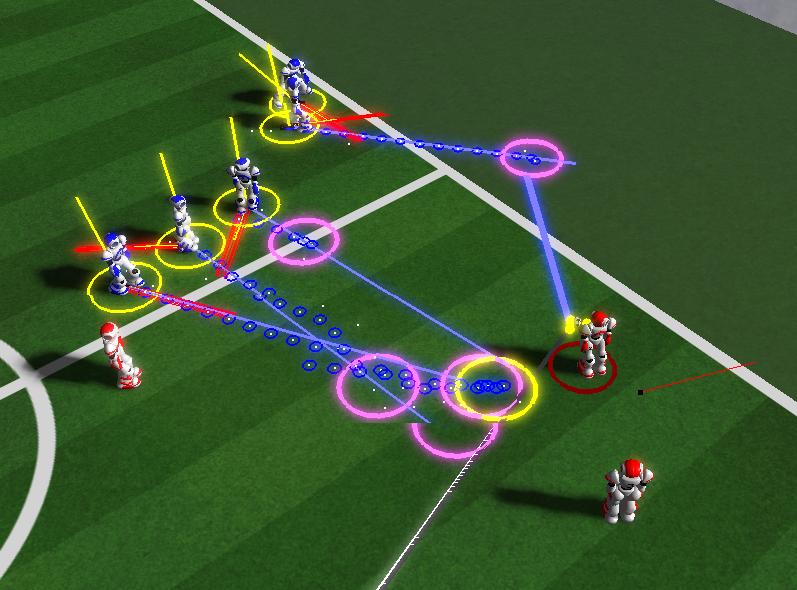
\includegraphics[scale=0.38]{figuras/roboviz.png}

\caption{Simulação em tempo real de agentes no Roboviz utilizando um plot gráfico para analisar comportamentos.} Fonte: \cite{robovizImg} \label{fig:roboviz}

\end{figure}
\FloatBarrier

\subsection{Times da Simulação 3D}

A liga de simulação 3D é composta por times que foram desenvolvidos por grupos de pesquisa de diversos países. A quantidade de
equipes que possuem times competitivos é pequena, isso se da pelo fato de que o desenvolvimento de uma equipe requer uma pesquisa
aprofundada sobre movimentação de agentes, protocolos de comunicação, planejamento e coordenação multi-agente e inteligência 
artificial distribuída.

Um dos fatores que facilitam grupos de pesquisa a se inserirem na competição, são os times base disponibilizados por equipes para
fomentar e estimular a pesquisa no ambito da robótica autônoma simulada. Como por exemplo, o MagmaOffenburg \cite{magma}, um time
base cedido para a comunidade científica.

Atualmente os principais times que participam da RoboCup podem ser visualizados na tabela \ref{tab:times}.

\begin{table}[h]

\scalefont{0.8}

\centering

\caption{Principais times que participam da RoboCup e sua Universidade.} Fonte: \cite{SimulationLeague} 

  \begin{tabular}{|c|c|}

    \hline
    \hline
    Time & Universidade \\
    \hline
    \hline
    Apollo3D & Nanjing University of Posts and Telecommunications \\
    \hline`
    AUA3D & Anhui University of Architecture \\
    \hline
    BahiaRT & Universidade do Estado da Bahia \\
    \hline
    Bold Heart & University of Hertfordshire \\
    \hline
    cit3d & Changzhou Institute of Technology \\
    \hline
    FCPortugal & University of Aveiro/University of Minho/University of Porto \\
    \hline
    FUT-K3D & Fukui University of Technology \\
    \hline
    HfutEngine3D & HFUT \\
    \hline
    ITAndroids & Instituto Tecnologico de Aeronautica \\
    \hline
    IUIM3D & Iran University of Industries Mines (Tehran Center Branch) \\
    \hline
    KarachiKoalas & University of Technology, Sydney and Institute of Business Administration, Karachi \\
    \hline
    KylinSky3D & Hohai University Wentian College / Hohai University \\
    \hline
    L3M-SIM & Paris8 University \\
    \hline
    magmaOffenburg & Hochschule Offenburg \\
    \hline
    Miracle3D & Hefei Normal University \\
    \hline
    Mithras3D & Farzanegan Tehran \\
    \hline
    Nexus3D & Ferdowsi University of Mashhad \\
    \hline
    ODENS & Osaka Electro-Communication University \\
    \hline
    Paydar3D & Sharif University Of Technology \\
    \hline
    Rightel & University of Tehran \\
    \hline
    RoboCanes & University of Miami \\
    \hline
    Scorpius & AmirKabir University of Technology (AUT) \\
    \hline
    SEU-Jolly & Southeast University \\
    \hline
    UTAustinVilla & University of Texas at Austin \\
    \hline
    \hline
  \end{tabular}

  \label{tab:times}
\end{table}


Além dos times base, os TDP(Team Description Paper) que são descrições de cada time e artigos sobre as metodologias empregadas
em seus times são divulgadas em simpósios e congressos, facilitando o trabalho de outras equipes e fomentando a melhoria contínua
de metodologias empregadas para resolver problemas em aberto.

Algumas das lacunas em aberto, como fazer com que os agentes corram, ou fazer com que agentes efetuem um passe de forma coordenada
e planejada, desviar de obstáculos móveis e atuarem em ambientes dinâmicos são lacunas que ainda estão em aberto e possuem  
metodologias em desenvolvimento. Um dos times que mais se aproximam do comportamento humano é o MagmaOffenburg, e sem sombra de dúvida, 
será um dos primeiros times a conseguir fazer com que o robô consiga correr.

A maioria dos times hoje utilizam uma movimentação omnidirecional e dinâmica, onde suas poses são calculadas e alcançadas através de 
modelos matemáticos utilizando cinemática inversa. Tais modelos substituiram a movimentação estática, que dificultava a realização de 
jogadas e comportamentos devido o fato de que o ambiente é dinâmico e contínuo. 


%\section{Futebol de robos e Simulacao 3D}
%  \subsection{Robocup}%o porque da robocup, como se organiza, as categorias
%  \subsection{Simulacao 3D}%simspark, roboviz, arquitetura, imagens ilustrando 
   %falar sobre os atuais times, suas principais abordagens e estado da arte, principais desafios ainda em aberto
   
%Porque os métodos baseados em amostra não são a solução para o planejamento de movimento humanóide

%\section{Planejamento em SMA}


%\section{Coordenaç~ao em SMA}
%O Futabol Robotico em geral e a liga de simulacao em particular, constituem dominios particularmente adequados a aplicacao da investigacao realizada em 
%metodologias de coordenacao em Sistemas Multi-Agente, nomeadamente no que diz respeito a coordenacao para agentes cooperativos.

%O dominio do futebol robotico e extremamente complexo, dinamico, parcialmente cooperativo e parcialmente adverso. Existem diversos tipos de coordenacao aplicados
%ao dominio do futebol robotico como:

%\begin{enumerate}
%\item Coordenacao por Comunicacao
%\item Coordenacao por Percepcao Inteligente
%\item Coordenacao por Modelizacao Mutua
%\item Coordenacao Estrategica
%\item Coordenacao Parcialmente Hierarquica
%\end{enumerate}

%A construção de agentes capazes de balancear a reatividade com a capacidade de deliberacao individual e social sao fundamentais para que os agentes realizem a cooperacao. O estado 
%do mundo de um agente estrategico e definido como uma estrutura multi-nivel contendo desde informacao de baixo nivel( incluindo as posicoes, velocidade e orientacoes dos objetos 
%presentes no mundo) ate informacao de nivel estrategico (incluindo informacao temporal estrategica que ira permitir a selecao de taticas a utilizar). Este estado de mundo e atualizado 
%utilizando informacao proveniente da percepcao do agente, das comunicacoes recebidas, da dinamica do mundo e da predicao dos efeitos das suas acoes e das acoes dos outros agentes.

%\section{Arquitetura dos Agentes}

%\subsection{Caracteristicas da simulacao}

%\subsection{Estado do Mundo}

%\subsection{Atualizacao do Estado do Mundo}

%\subsection{Predicao dos Efeitos das Acoes}

%\section{Prediçao do Colisao}
